%%%%%%%%%%%%%%%%%%%%%%%%%%%%%%%%%%%%%%%%%
% The Legrand Orange Book
% LaTeX Template
% Version 2.4 (26/09/2018)
%
% This template was downloaded from:
% http://www.LaTeXTemplates.com
%
% Original author:
% Mathias Legrand (legrand.mathias@gmail.com) with modifications by:
% Vel (vel@latextemplates.com)
%
% License:
% CC BY-NC-SA 3.0 (http://creativecommons.org/licenses/by-nc-sa/3.0/)
%
% Compiling this template:
% This template uses biber for its bibliography and makeindex for its index.
% When you first open the template, compile it from the command line with the 
% commands below to make sure your LaTeX distribution is configured correctly:
%
% 1) pdflatex main
% 2) makeindex main.idx -s StyleInd.ist
% 3) biber main
% 4) pdflatex main x 2
%
% After this, when you wish to update the bibliography/index use the appropriate
% command above and make sure to compile with pdflatex several times 
% afterwards to propagate your changes to the document.
%
% This template also uses a number of packages which may need to be
% updated to the newest versions for the template to compile. It is strongly
% recommended you update your LaTeX distribution if you have any
% compilation errors.
%
% Important note:
% Chapter heading images should have a 2:1 width:height ratio,
% e.g. 920px width and 460px height.
%
%%%%%%%%%%%%%%%%%%%%%%%%%%%%%%%%%%%%%%%%%

%----------------------------------------------------------------------------------------
%	PACKAGES AND OTHER DOCUMENT CONFIGURATIONS
%----------------------------------------------------------------------------------------

\documentclass[14pt,fleqn]{book} % Default font size and left-justified equations

\input{_includes/structure.tex} 
\usepackage[european]{circuitikz}
\hypersetup{pdftitle={Laser Tracking - Embedded PID Controller - Technical Documentation},pdfauthor={Julien VILLEMEJANE}} % Uncomment and fill out to include PDF metadata for the author and title of the book

%----------------------------------------------------------------------------------------
%\addto\captionsenglish{\renewcommand{\contentsname}{Ce que vous trouverez dans cet ouvrage...}}
\begin{document}

%----------------------------------------------------------------------------------------
%	TITLE PAGE
%----------------------------------------------------------------------------------------

\begingroup
\thispagestyle{empty} % Suppress headers and footers on the title page
\begin{tikzpicture}[remember picture,overlay]
\node[inner sep=0pt] (background) at (current page.center) {\includegraphics[width=\paperwidth]{global_pictures/background2.pdf}};
\draw (current page.center) node [fill=ocre!30!white,fill opacity=0.6,text opacity=1,inner sep=1cm]{\Huge\centering\bfseries\sffamily\parbox[c][][t]{\paperwidth}{\centering Laser Tracking - Embedded PID Controller\\[15pt] % Book title
{\Large Technical Documentation}\\[20pt] % Subtitle
\color{ocre!80!black} {\Large  Julien VILLEMEJANE} \\ \large version 2021}}; % Author name
\end{tikzpicture}
\vfill
\begin{center}
	\includegraphics[width=8cm]{global_pictures/LEnsE_logo.pdf}
\end{center}
\endgroup

%----------------------------------------------------------------------------------------
%	COPYRIGHT PAGE
%----------------------------------------------------------------------------------------

\newpage
~\vfill
\thispagestyle{empty}

\noindent \copyright\ 2020 LEnsE - Laboratoire d'Enseignement Expérimental\\ % Copyright notice

\noindent The \textbf{embedded PID controller system} presented in this document was designed and realized at the LEnsE lab of \textsc{Institut d'Optique Graduate School / France} by \textbf{Cyrille DES COGNETS, Théo MARTIN and Igor RESHETNIKOV} (MSc 1 students) and supervised by \textbf{Caroline KULCSAR and Julien VILLEMEJANE}, with the precious help of Thierry AVIGNON and Cédric LEJEUNE.\\ 

\noindent It was designed for a previous existing didactic demonstrator of a 2D tracking of a laser beam, developped by \textbf{Caroline KULCSAR, Fabienne BERNARD and Thierry AVIGNON}.\\
% Publisher

\noindent \textsc{lense.institutoptique.fr}\\ % URL

\noindent Licensed under the Creative Commons Attribution-NonCommercial 3.0 Unported License (the ``License''). You may not use this file except in compliance with the License. You may obtain a copy of the License at \url{http://creativecommons.org/licenses/by-nc/3.0}. Unless required by applicable law or agreed to in writing, software distributed under the License is distributed on an \textsc{``as is'' basis, without warranties or conditions of any kind}, either express or implied. See the License for the specific language governing permissions and limitations under the License.\\ % License information, replace this with your own license (if any)

\begin{center}
	\includegraphics[width=8cm]{global_pictures/LEnsE_logo.pdf}
\end{center}

%----------------------------------------------------------------------------------------
%	TABLE OF CONTENTS
%----------------------------------------------------------------------------------------

%\usechapterimagefalse % If you don't want to include a chapter image, use this to toggle images off - it can be enabled later with \usechapterimagetrue

\chapterimage{global_pictures/chapter_head_1.pdf} % Table of contents heading image

\pagestyle{empty} % Disable headers and footers for the following pages

\tableofcontents % Print the table of contents itself

\cleardoublepage % Forces the first chapter to start on an odd page so it's on the right side of the book

\pagestyle{fancy} % Enable headers and footers again


%----------------------------------------------------------------------------------------
%	PART
%----------------------------------------------------------------------------------------
%% %% 
\part{2D Tracking of a Laser Beam}
%%
\chapter{Presentation of the initial system}\index{Laser Tracking}

Laser tracking and adaptative optics
%
\section{Laser Beam Tracking}

Presentation of the existing system 

%
\section{Materials}\index{Previous PID experience}

Details about the different blocks

\subsection{Actuators and control}

Motors and specification

\subsection{Detector and signal}

4Q photodiode and electronic circuit

%
\section{Operationnal steps}

Open Loop and step response

Controller 

%%
\chapter{Mathematical model of the loop}\index{System model}

\section{Second order model}

Model of the system

Estimation of the parameters

\section{Simulink\textregistered{} simulation}

Some simulations in open loop and with or without PID controller

%%
\chapter{From Analog to Digital PID control}

In continous time

Move to digital world : adding ADC and DAC, numerical controller, sampling frequency...

%% %% 
\part{Embedded PID Controller}
%% 
\chapter{Introduction and goals}

The analog version of the PID controller was sufficient to explore the basics of closed-loop system and all the stability issues it can appear when you want to control a system.

But one of the \textbf{limitation} of this controller was the fact that PID coefficients values injected in the controller are not displayed. As a system engineer, it's necessary to compare the prediction of a simulated model and the real experiment. 

Additionally, the controller model is \textbf{limited to PID}. It's not possible to compare to new kind of controllers based on the state of the system or/and predictive models as Linear Quadratic Gaussian control. 

A way to answer to the two problems mentionned here is to use a digital controller where you can adapt "on-the-fly" the running code.

\section{Test}
Bla bla bla

\section{Materials}

A \textbf{L476RG Nucleo board} from \textit{STMicroelectronics} is used to perform the embedded calculations and data acquisition on the two channels (X and Y axis). The program is developped with \textbf{MBED OS} (version 2) and the \textbf{mbed-dsp} library (Digital Signal Processing specific functions are available in this library).

An \textbf{electronic board} was designed to adapt the voltages from the detector to the analog-to-digital converter and from the digital-to-analog converter to the motor controller. 

An interface to specify the coefficients values was developped with MATLAB\textregistered{} Application Designer\footnote{This application was tested on Windows, but should also work on Linux and Mac. But a MATLAB\textregistered{} licence is required. The application was developped with the R2020b version of MATLAB\textregistered{}.}. The coefficients are sended from the computer to the embedded board by a RS232 protocol that is virtualized in an USB connexion.

\section{Voltage adaptation board}



%% 
\chapter{Differents modes of operation}

\section{Controlling a system step-by-step}

Connexion

Alignment

Motor control

Step Response (or frequency response) - Open Loop model

PID Control



%% 
\chapter{Communication protocol}

To transmit data from the embedded controller to the computer and in the other direction, a R\textbf{S232 (serial) transmission} is used. A virtual communication port is established inside an USB connexion between the board and the computer.

A high-level protocol was established to run the embedded system in the differents working mode specified in the previous chapter. This chapter explains the protocol used between the board - i.e. the embedded controler - and the host system - i.e. the computer.

\section{Basic Communication Mode}

The embedded PID controller uses a \textbf{textual data packet} based protocol to communicate with the host system. A communication \textbf{session is always initialized by the host system}. No data are sended by the board after powering up.

A data packet sended by the host system is called a \textbf{Request}. Once the board receives a request, it will reply the host system with data packets called \textbf{Responses} (see the figure~\ref{fig:rs232_RSR_mode}).

\begin{figure}[h!]
\centering
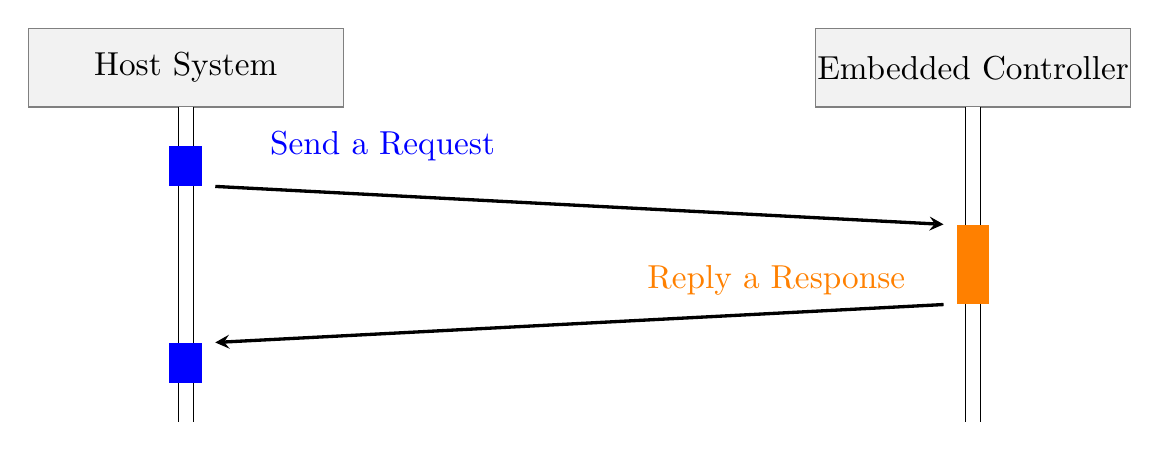
\begin{tikzpicture}
	\draw [gray, fill=gray, fill opacity=.1] (0,0) rectangle (4,-1);
	\draw (2,-0.5) node[scale=1.2] {Host System};
	\draw [double distance = 5pt] (2,-1) -- (2,-5);
	\draw [gray, fill=gray, fill opacity=.1] (10,0) rectangle (14,-1);
	\draw (12,-0.5) node[scale=1.2] {Embedded Controller};
	\draw [double distance = 5pt] (12,-1) -- (12,-5);	
	
	\draw [blue, fill=blue] (1.8,-1.5) rectangle (2.2,-2);
	\draw (4.5,-1.5) node[scale=1.2,text=blue] {Send a Request};
	\draw[very thick,->,shorten >=5pt,shorten <=5pt,>=stealth] (2.2,-2) -- (11.8,-2.5);
	
	\draw [orange, fill=orange] (11.8,-2.5) rectangle (12.2,-3.5);
	\draw (9.5,-3.2) node[scale=1.2,text=orange] {Reply a Response};
	\draw[very thick,->,shorten >=5pt,shorten <=5pt,>=stealth] (11.8,-3.5) -- (2.2,-4);
	\draw [blue, fill=blue] (1.8,-4) rectangle (2.2,-4.5);
\end{tikzpicture}
\caption{Embedded Controller communication : Request/Simple Response Mode} \label{fig:rs232_RSR_mode}
\end{figure}

\begin{remark}
All the packets must end by a CR/LF terminator ("carriage return" and "linefeed").
\end{remark}

\section{Connexion and Stop Mode}\index{Mode Stop}

When the serial connexion is setup by the host system, a stop request is sended from the host to the board. The board doesn't send any response in this case.

The stop request packet is : 

\begin{center}
\textbf{\color{blue}\large O\_!\textbackslash{}r\textbackslash{}n}
\end{center}


\begin{figure}[h!]
\centering
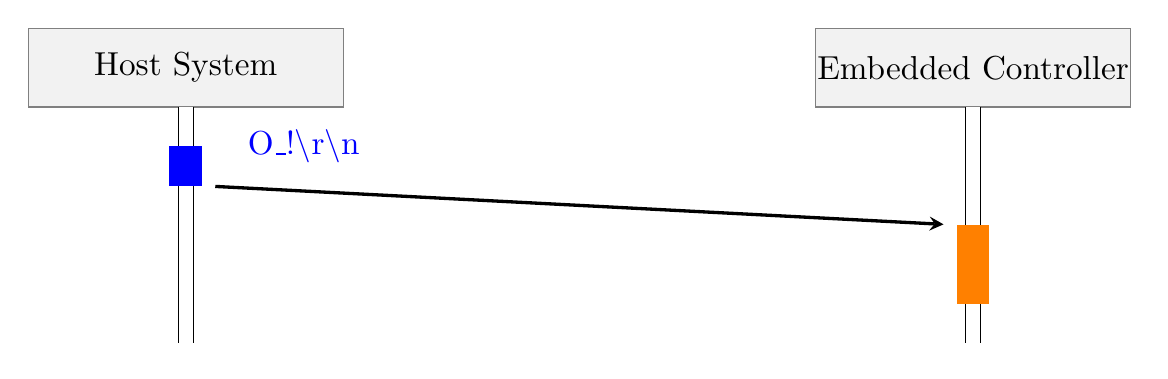
\begin{tikzpicture}
	\draw [gray, fill=gray, fill opacity=.1] (0,0) rectangle (4,-1);
	\draw (2,-0.5) node[scale=1.2] {Host System};
	\draw [double distance = 5pt] (2,-1) -- (2,-4);
	\draw [gray, fill=gray, fill opacity=.1] (10,0) rectangle (14,-1);
	\draw (12,-0.5) node[scale=1.2] {Embedded Controller};
	\draw [double distance = 5pt] (12,-1) -- (12,-4);	
	
	\draw [blue, fill=blue] (1.8,-1.5) rectangle (2.2,-2);
	\draw (3.5,-1.5) node[scale=1.2,text=blue] {O\_!\textbackslash{}r\textbackslash{}n};
	\draw[very thick,->,shorten >=5pt,shorten <=5pt,>=stealth] (2.2,-2) -- (11.8,-2.5);
	
	\draw [orange, fill=orange] (11.8,-2.5) rectangle (12.2,-3.5);	
\end{tikzpicture}
\caption{Embedded Controller communication : Stop Mode} \label{fig:rs232_alignment_mode}
\end{figure}

\section{Alignment Mode}\index{Mode Alignment}

The alignment mode permits to align the optical banch, including laser system, motors and detectors. In this mode, the two motors (X and Y axis) are positionned in the center of the functionnal range. The board collects \textbf{datas from the two detectors} and sends them to the host system \textbf{ten times per second}.

\medskip

The alignment mode request packet is : 

\begin{center}
\textbf{\color{blue}\large A\_!\textbackslash{}r\textbackslash{}n}
\end{center}

The alignment mode response packet is : 

\begin{center}
\textbf{\color{orange}\large A\_Xvalue\_Yvalue\_!\textbackslash{}r\textbackslash{}n}
\end{center}


\medskip

where \textit{\color{orange}Xvalue} is the adapted voltage of the detector on X axis, i.e. the position of the beam on the X axis, and \textit{\color{orange}Yvalue} is the adapted voltage of the detector on Y axis, i.e. the position of the beam on the Y axis.

\textit{\color{orange}Xvalue} and \textit{\color{orange}Yvalue} are two real numbers (\textit{double} type in C).

Response packets are sending ten times per second by the board, until a stop request is sended.

\begin{figure}[h!]
\centering
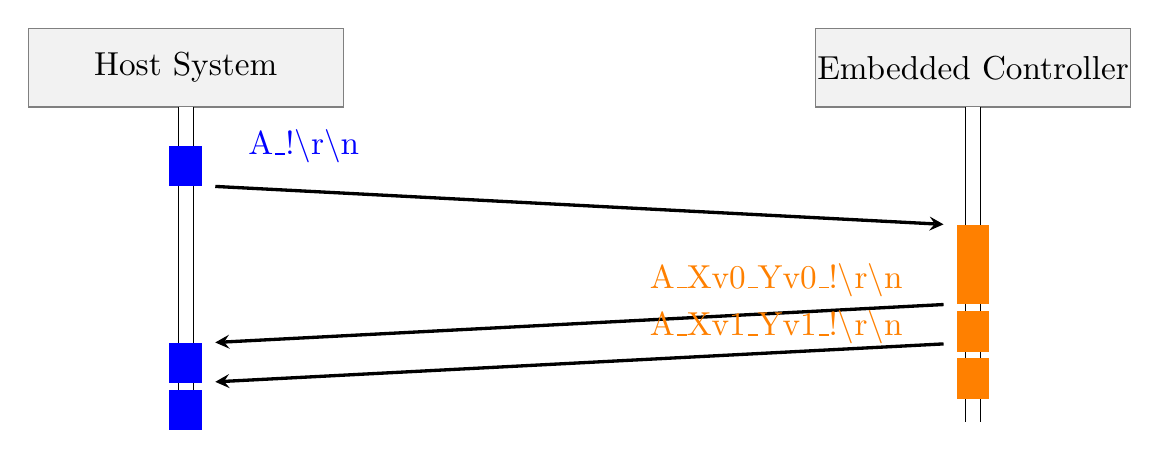
\begin{tikzpicture}
	\draw [gray, fill=gray, fill opacity=.1] (0,0) rectangle (4,-1);
	\draw (2,-0.5) node[scale=1.2] {Host System};
	\draw [double distance = 5pt] (2,-1) -- (2,-5);
	\draw [gray, fill=gray, fill opacity=.1] (10,0) rectangle (14,-1);
	\draw (12,-0.5) node[scale=1.2] {Embedded Controller};
	\draw [double distance = 5pt] (12,-1) -- (12,-5);	
	
	\draw [blue, fill=blue] (1.8,-1.5) rectangle (2.2,-2);
	\draw (3.5,-1.5) node[scale=1.2,text=blue] {A\_!\textbackslash{}r\textbackslash{}n};
	\draw[very thick,->,shorten >=5pt,shorten <=5pt,>=stealth] (2.2,-2) -- (11.8,-2.5);
	
	\draw [orange, fill=orange] (11.8,-2.5) rectangle (12.2,-3.5);
	\draw (9.5,-3.2) node[scale=1.2,text=orange] {A\_Xv0\_Yv0\_!\textbackslash{}r\textbackslash{}n};
	\draw[very thick,->,shorten >=5pt,shorten <=5pt,>=stealth] (11.8,-3.5) -- (2.2,-4);
	\draw [blue, fill=blue] (1.8,-4) rectangle (2.2,-4.5);

	\draw [orange, fill=orange] (11.8,-3.6) rectangle (12.2,-4.1);
	\draw (9.5,-3.8) node[scale=1.2,text=orange] {A\_Xv1\_Yv1\_!\textbackslash{}r\textbackslash{}n};
	\draw[very thick,->,shorten >=5pt,shorten <=5pt,>=stealth] (11.8,-4) -- (2.2,-4.5);
	\draw [blue, fill=blue] (1.8,-4.6) rectangle (2.2,-5.1);
	\draw [orange, fill=orange] (11.8,-4.2) rectangle (12.2,-4.7);
	
\end{tikzpicture}
\caption{Embedded Controller communication : Alignment Mode} \label{fig:rs232_alignment_mode}
\end{figure}


\section{Motor Control Mode}\index{Mode Motor Control}

The motor mode permits to \textbf{control the two axis motors independently}, in the whole range of operation, to determine the maximum deviation allowed to the beam to stay on the detector. The desired position is sended by the host system by a request packet. The board collects \textbf{datas from the two detectors} and sends them to the host system \textbf{three times per second}.

\medskip

The motor mode request packet is : 

\begin{center}
\textbf{\color{blue}\large M\_Xpos\_Ypos\_!\textbackslash{}r\textbackslash{}n}
\end{center}

\medskip

where \textit{\color{blue}Xpos} and \textit{\color{blue}Ypos} is the desired position given as a pourcentage of the whole possible deviation. \textit{\color{blue}Xpos} and \textit{\color{blue}Ypos} are two real numbers (\textit{double} type in C).

\medskip


The motor mode response packet is : 

\begin{center}
\textbf{\color{orange}\large M\_Xpos\_Ypos\_Xdet\_Ydet\_!\textbackslash{}r\textbackslash{}n}
\end{center}


\medskip

where \textit{\color{orange}Xpos} and \textit{\color{orange}Ypos} are the position of the motors given as a pourcentage of the whole possible deviation, \textit{\color{orange}Xdet} is the adapted voltage of the detector on X axis, i.e. the position of the beam on the X axis, and \textit{\color{orange}Ydet} is the adapted voltage of the detector on Y axis, i.e. the position of the beam on the Y axis. 

\textit{\color{orange}Xpos}, \textit{\color{orange}Ypos}\textit{\color{orange}Xvalue}, \textit{\color{orange}Yvalue} are real numbers (\textit{double} type in C).

Response packets are sending \textbf{three times per second} by the board, until a stop request is sended.

\begin{figure}[h!]
\centering
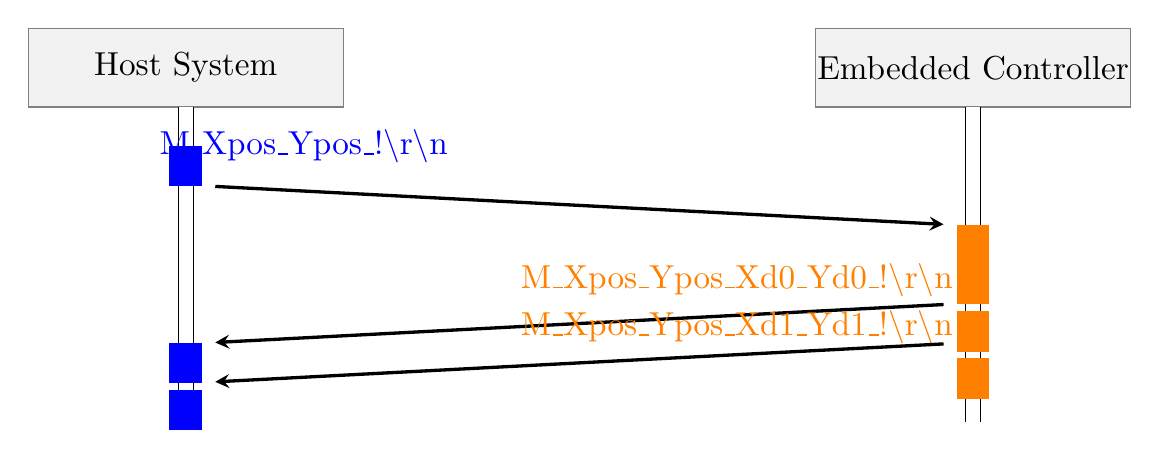
\begin{tikzpicture}
	\draw [gray, fill=gray, fill opacity=.1] (0,0) rectangle (4,-1);
	\draw (2,-0.5) node[scale=1.2] {Host System};
	\draw [double distance = 5pt] (2,-1) -- (2,-5);
	\draw [gray, fill=gray, fill opacity=.1] (10,0) rectangle (14,-1);
	\draw (12,-0.5) node[scale=1.2] {Embedded Controller};
	\draw [double distance = 5pt] (12,-1) -- (12,-5);	
	
	\draw [blue, fill=blue] (1.8,-1.5) rectangle (2.2,-2);
	\draw (3.5,-1.5) node[scale=1.2,text=blue] {M\_Xpos\_Ypos\_!\textbackslash{}r\textbackslash{}n};
	\draw[very thick,->,shorten >=5pt,shorten <=5pt,>=stealth] (2.2,-2) -- (11.8,-2.5);
	
	\draw [orange, fill=orange] (11.8,-2.5) rectangle (12.2,-3.5);
	\draw (9,-3.2) node[scale=1.2,text=orange] {M\_Xpos\_Ypos\_Xd0\_Yd0\_!\textbackslash{}r\textbackslash{}n};
	\draw[very thick,->,shorten >=5pt,shorten <=5pt,>=stealth] (11.8,-3.5) -- (2.2,-4);
	\draw [blue, fill=blue] (1.8,-4) rectangle (2.2,-4.5);

	\draw [orange, fill=orange] (11.8,-3.6) rectangle (12.2,-4.1);
	\draw (9,-3.8) node[scale=1.2,text=orange] {M\_Xpos\_Ypos\_Xd1\_Yd1\_!\textbackslash{}r\textbackslash{}n};
	\draw[very thick,->,shorten >=5pt,shorten <=5pt,>=stealth] (11.8,-4) -- (2.2,-4.5);
	\draw [blue, fill=blue] (1.8,-4.6) rectangle (2.2,-5.1);
	\draw [orange, fill=orange] (11.8,-4.2) rectangle (12.2,-4.7);
	
\end{tikzpicture}
\caption{Embedded Controller communication : Motor Mode} \label{fig:rs232_motor_mode}
\end{figure}

\section{Open-Loop Mode}\index{Mode Open-Loop}



%#define N_SAMPLES   256
%
%sscanf(g_value, "S_%lf_%lf_%lf_%lf_%lf_!\r\n", &sX_min, &sX_max, &sY_min, &sY_max, &g_sampling_frequency);
%
%            for(int i=0; i < N_SAMPLES; i++){
%                pc.printf("S_x_%d_%lf_!\r\n", i+1, samplesX[i]);
%                wait_ms(10);
%                pc.printf("S_y_%d_%lf_!\r\n", i+1, samplesY[i]);
%                wait_ms(10);
%                pc.printf("S_s_%d_%lf_!\r\n", i+1, samplesSTEP[i]);
%                wait_ms(10);
%            }
%            pc.printf("S_END_!\r\n");

\section{PID Controller Mode}\index{Mode PID Controller}

%sscanf(g_value, "D_%lf_%lf_%lf_%lf_%lf_%lf_%lf_!\r\n", &g_Kpx, &g_Kpy, &g_Kix, &g_Kiy, &g_Kdx, &g_Kdy, &g_sampling_frequency);
%
%pc.printf("%c_OK! gX = %lf gY = %lf Fe = %lf\r\n", mode, g_Kpx, g_Kpy, g_sampling_frequency);

%% 
\chapter{Embedded program in a microcontroller}

\section{Overview}

A \textbf{L476RG Nucleo Board}, including a \textit{STMicroelectronics} STM32 ARM core, is used to :
\begin{itemize}
	\item perform the real-time PID control of the system ;
	\item transfer data from and to the host system (computer).
\end{itemize}

\begin{figure}[!h]
	\centering
	\includegraphics[width=12cm]{images/nucleo.jpg}
	\caption{Nucleo Board, STMicroelectronics}
	\label{fig:nucleoBoard}
\end{figure}

The program is written for the \textbf{MBED OS 2 compiler}.



\section{RS232 Communication and protocol execution}

\section{Real-time operations}


%% 
\chapter{MATLAB\textregistered{} Application}

\section{Overview}

\section{Interface Design}

\section{RS232 Communication and protocol execution}




% CONTENTS
%\input{_includes/template_content.tex}



%----------------------------------------------------------------------------------------
%	BIBLIOGRAPHY
%----------------------------------------------------------------------------------------

%\chapter*{Bibliography}
%\addcontentsline{toc}{chapter}{\textcolor{ocre}{Bibliography}} % Add a Bibliography heading to the table of contents

%------------------------------------------------

%\section*{Articles}
%\addcontentsline{toc}{section}{Articles}
%\printbibliography[heading=bibempty,type=article]

%------------------------------------------------

%\section*{Books}
%\addcontentsline{toc}{section}{Books}
%\printbibliography[heading=bibempty,type=book]

%----------------------------------------------------------------------------------------
%	INDEX
%----------------------------------------------------------------------------------------

\cleardoublepage % Make sure the index starts on an odd (right side) page
\phantomsection
\setlength{\columnsep}{0.75cm} % Space between the 2 columns of the index
\addcontentsline{toc}{chapter}{\textcolor{ocre}{Index}} % Add an Index heading to the table of contents
\printindex % Output the index

%----------------------------------------------------------------------------------------

\end{document}
